\documentclass[../main]{subfiles}

\graphicspath{{../figures/}}

\begin{document}

\chapter{序論}
\label{cp:introduction}
\thispagestyle{empty}
\minitoc
\newpage

\section{背景}
\label{sec:intro_background}

近年，パラリンピックへの社会的関心の高まりとともにパラスポーツの競技レベルは著しく向上しており，経験則のみならず科学的知見に基づいたトレーニング支援の需要が急増している\citeja{nakamori}．スポーツ科学やバイオメカニクスの分野において，パフォーマンス向上のための指導指針を構築する際，最も標準的なアプローチは一般化である．これは，多数の熟練者の動作データを収集・統計処理し，万人に共通する理想的なフォームや身体操作の標準モデルを導き出そうとする試みであり，健常者を対象とした多くの競技において成功を収めてきた\citeen{leesTechniqueAnalysisSports2002}．


一方，車椅子卓球をはじめとするパラスポーツの領域においては，この身体機能の多様性を管理し，競技の公平性を担保するために国際パラリンピック委員会（IPC）によって科学的根拠に基づくクラス分けの導入が推進されてきた\citeen{tweedyInternationalParalympicCommittee2011}．これは医学的診断のみならず，障害が競技パフォーマンスに与える影響の程度に基づいて選手をカテゴライズする手法で競技の公平性を確保している．

しかし，このクラス分けシステムはあくまでも競技の公平性を担保するための区分であり，同一のクラス内の選手間での身体操作の均質性までを保証するものではない．実際，車椅子卓球選手の筋活動を解析した先行研究においても，同一の障害クラスに属する選手間であっても，脊髄損傷の完全・不全といった障害の程度によって，打球動作時の筋活動パターンや発火タイミングに明確な差異が存在することが報告されている\citeen{norouziElectromyographicAnalysisElite2025}.例えば，体幹制御や上肢の運動戦略は，残存機能のわずかな違いによって大きく異なるため，集団の平均値を用いた解析では，各選手が独自に獲得した代償動作や最適化された運動戦略がノイズとして処理されてしまうリスクがある．

このように身体機能の極端な多様性が存在する状況下では，クラス分けによる大まかなグルーピングを前提としつつも，パフォーマンスの最大化を目指す指導現場においては，既存の一般化のアプローチには限界があると言わざるを得ない．したがって，パラアスリートのパフォーマンスを最大化するためには，各選手固有の残存機能に立脚した個別最適化のアプローチも考慮する必要がある．



%文献の引用例はこのようになる\citeja{cao2014main1-1-4-3}，\citeen{Kiribayashi2018}，\citeen{kingma2017Adam}，\citeen{tang2021cause}，\citeen{Zacny2010}．

%すべての図表は必ず本文中で引用して説明する．
%図表の例：コーンペネトロメータを\reffig{fig:cone_penetrometer}に示す．\reftab{tab:traffic_cone_index}が示すように，各建設機械の走行に必要とされているコーン指数は既にわかっている．




% \begin{figure}[t]
%   \centering
%   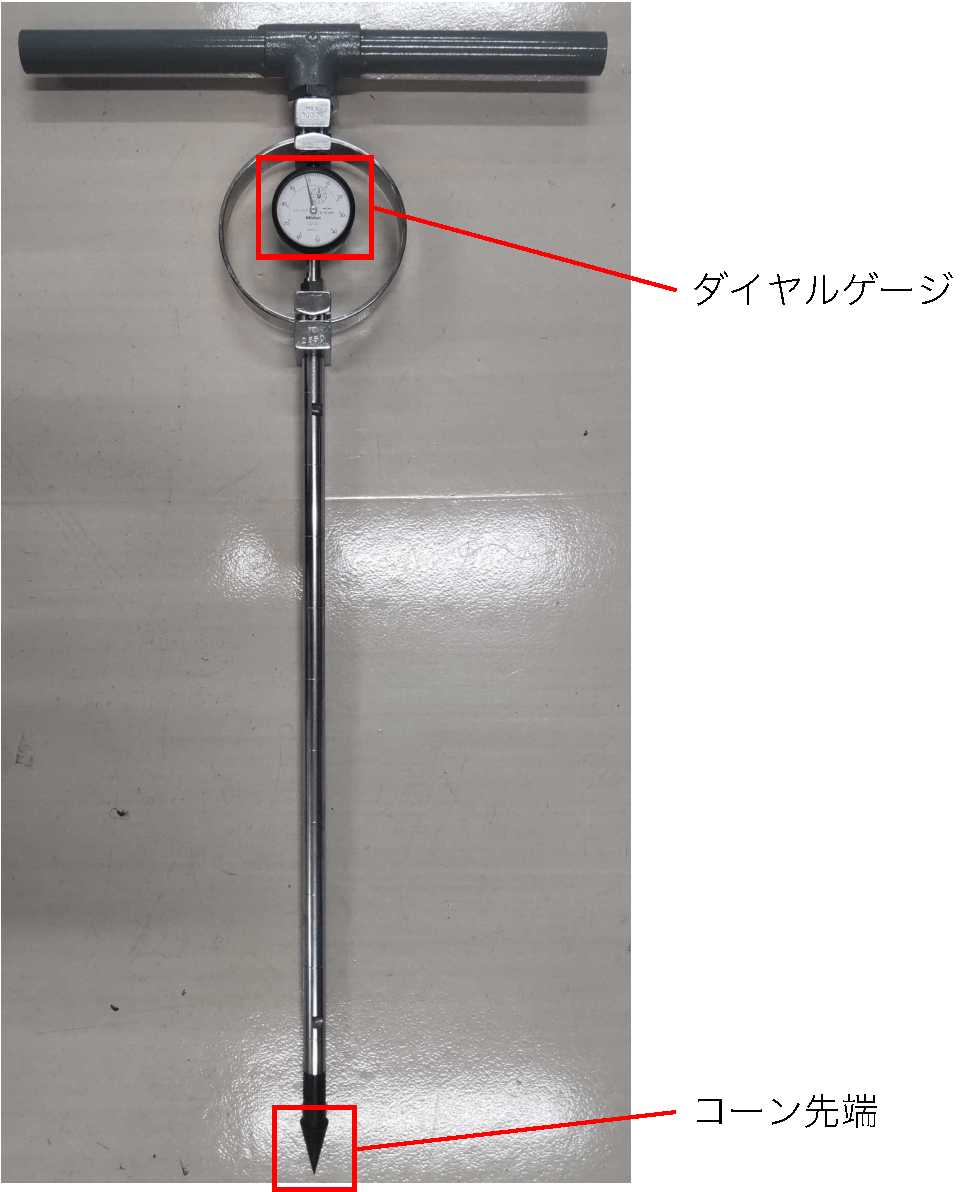
\includegraphics[keepaspectratio, width=0.5\linewidth]{chap1/cone_penetrometer.pdf}
%   \caption{コーンペネトロメータ}
%   \label{fig:cone_penetrometer}
% \end{figure}

% % textlint-disable

% \vspace{3\zh}
% \begin{table}[t]
%   \caption{走行に必要なコーン指数（\protect\citeja{maff2015}を基に作成）}
%   \label{tab:traffic_cone_index}
%   \centering
%   \begin{tabular}{cc}
%     \toprule
%     建設機械の種類                      & コーン指数[\unit{\kN/\m^2}] \\
%     \midrule
%     超湿地ブルドーザー                    & 200以上                \\
%     湿地ブルドーザー                     & 300以上                \\
%     普通ブルドーザー（\qty{15}{\tonne}級程度） & 500以上                \\
%     普通ブルドーザー（\qty{21}{\tonne}級程度） & 700以上                \\
%     スクレープドーザ                     & 600以上                \\
%                                  & （超湿地型は400以上）         \\
%     被けん引式スクレーパ（小型）               & 700以上                \\
%     自走式スクレーパ（小型）                 & 1,000以上              \\
%     ダンプトラック                      & 1,200以上              \\
%     \bottomrule
%   \end{tabular}
% \end{table}

% textlint-enable

\clearpage

\section{先行研究}
\label{sec:intro_previous-research}

\subsection{健常者及び車椅子卓球の打球動作のバイオメカニクス研究}
\label{sec:intro_previous-research_1}

卓球競技は高速かつ精緻なラケット操作が求められる競技であり，そのパフォーマンスを支える身体動作については，健常者を対象とした多くのバイオメカニクス研究が蓄積されている．
例えば，Heらは，卓球のフォアハンドトップスピン打法における下肢のバイオメカニクスに関するシステマティックレビューを行い，打球動作における床反力や関節モーメントの重要性を報告している\citeen{heLowerLimbBiomechanics2022}．
しかし，車椅子卓球選手，特に座位クラスの選手においては，下肢や体幹機能に制約があるため，これらの健常者モデルをそのまま適用することはできない．

車椅子卓球を対象とした研究も近年増加傾向にある．
Zemkováらは，パラ卓球選手を対象に脊柱の可動域と体幹の回旋速度を計測し，体幹機能の制限がスイング速度生成に与える影響を定量的に分析した\citeen{zemkovaAssociationTrunkRotational2018}．
また，Kongらは，重度の下肢障害を持つ立位クラスのパラ卓球選手を対象としたケーススタディを行い，動作解析システムを用いて肩関節のバイオメカニクスを詳細に分析した\citeen{kongShoulderBiomechanicsParatable2022}．
さらに，Yamらは，慣性計測装置（IMU）を用いて車椅子および健常者卓球選手のフォアハンド・バックハンドドライブ時の上肢キネマティクスを計測し，障害の有無によるスイング軌道の差異を定量化している\citeen{yamMeasuringUpperLimb2021}．
また，三浦らが画像解析を用いた卓球フォアハンド打法における上肢動作の定量評価手法を提案しており，動作解析技術の応用が進められている\citeja{SanPuZhuoQiuhuoahandoDaFaniokeruShangZhiDongZuonoDingLiangPingJiaShouFanoTiAn2021}．

これらの先行研究は，主にモーションキャプチャやIMUセンサを用いた動作・姿勢の解析に主眼を置いている．
動作の結果として現れるフォームの違いを記述することには成功しているものの，その動作を生み出す駆動源である筋活動とパフォーマンスの関係性にまで踏み込んだ研究は限定的である．
また，多くの研究がスマッシュや特定の素振り動作といった単発の動作を対象としており，実際の試合で重要となる一度打った後の次の打球への準備や連続的なラリー動作の文脈を考慮した解析は十分になされていないのが現状である．

\subsection{表面筋電図を用いた運動解析と打球精度の評価}
\label{sec:intro_previous-research_2}

動作のメカニズムを解明するためには，身体の動きだけでなく，その原因となる筋活動を評価することが重要である．
表面筋電図は，非侵襲的に筋活動のタイミングや強度を計測できるため，スポーツ動作の評価に広く用いられている．

球技における打球精度と筋活動の関係については，Ikenagaら\citeen{ikenagaInfluenceBallImpact2020}の研究が挙げられる．
彼らはテニスのフォアハンドストロークにおいて，打球位置の変化がラケットのキネマティクスおよび前腕筋群の活動に与える影響を調査し，適切なインパクト位置と筋活動の協調がショット精度（Shot Accuracy）に寄与することを示唆している．
このように，パフォーマンスの結果と筋活動を紐づけるアプローチは有効であるが，車椅子卓球においては未だ十分な知見が得られていない．

車椅子卓球における数少ない筋電解析の例として，Norouziら\citeen{norouziElectromyographicAnalysisElite2025}の研究がある．
彼らは，脊髄損傷を持つエリートパラ卓球選手を対象に，損傷が完全か不全かによって，フォアハンドおよびバックハンド打法時の筋活動パターンに有意な差があることを明らかにした．
この研究は，同一の障害クラス内であっても，残存機能の詳細によって身体操作戦略が異なることを示しており，本研究が主張する個別最適化の必要性を強く裏付けるものである．
しかし，同研究においても，打球の成功・失敗という結果指標との直接的な因果関係までは言及されておらず，指導現場で即座に活用できる筋活動パターンの特定には至っていない．

\subsection{時系列データを考慮した機械学習による解析手法}
\label{subsec:related_ml}

\subsubsection{従来の統計的手法から時系列解析へ}
前節で述べたような筋活動解析において，従来は計測された時系列信号に対して整流や平滑化処理を施した後，積分筋電図や二乗平均平方根といった指標を用いて，特定区間における平均的な活動量や最大活動値を算出する手法が一般的であった．
その後，t検定や分散分析を用いて条件間の有意差を検定するというアプローチが主流である．

しかし，このような従来の手法には，高速かつ連続的なスポーツ動作を解析する上で限界がある．
それは，時系列信号を単一のスカラ値に要約する過程で，時間的な変化の情報が失われてしまうという点である．
卓球のラリーのような運動においては，単に筋肉がどれくらい強く活動したかという強度情報だけでなく，いつ活動を開始し，どのように協調して変化したかという時間的なパターンがパフォーマンスに決定的な影響を与える．
そのため，時系列データを情報の欠落なく，その動的な特徴を保持したまま学習し，打球の成否（IN/OUT）を分けるパターンを高精度に識別，比較できる機械学習モデルの導入が必要となる．

\subsubsection{Long Short Term Memory（LSTM）による筋活動パターンの学習}

上述した時系列性の問題を解決するために，近年スポーツバイオメカニクスや生体信号処理の分野では，深層学習を用いた解析手法が導入されている．
特に，再帰型ニューラルネットワーク（RNN）の一種であるLong Short Term Memory（LSTM）は，時系列データの解析において極めて有効な手法として知られている．

一般的なニューラルネットワークが各時点の入力を独立して処理するのに対し，LSTMは内部にゲート構造を持つメモリセルを有しており，過去の入力情報を保持しながら現在の処理を行うことができる．
これにより，長いシーケンスデータに含まれる長期的な依存関係を学習することが可能である．
筋電図解析の分野においても，Phinyomarkらが筋電信号を用いたジェスチャ認識に深層学習を適用し，従来の特徴量抽出に基づく手法よりも高い認識精度とロバスト性を達成している\citeen{phinyomarkEMGPatternRecognition2018}．
本研究のような連続ラリー動作においては，現在の打球動作が直前の打球からの戻り動作や準備動作といった過去の文脈に強く依存しているため，この時系列的な依存関係をモデル化できるLSTMは最適な手法と言える．

\subsubsection{Permutation Feature Importance（PFI）によるモデルの解釈と重要筋の特定}
LSTMのような深層学習モデルは，高い予測精度を誇る一方で，その判断プロセスが人間には理解しにくいブラックボックス性を持つことが課題とされる．
スポーツの指導現場に知見を還元するためには，単にAIが打球の成否を高精度に予測できたという事実だけでなく，なぜ成功（または失敗）と判断されたのか，すなわちどの筋肉の活動がその結果に寄与したのかを説明できなければならない．

この課題に対し，モデルに依存しない特徴量重要度の算出手法としてPermutation Feature Importance（PFI）が有用である．
PFIは，学習済みモデルの予測精度を基準として，ある特定の特徴量（本研究では特定の筋肉のデータ）の値をランダムにシャッフルした際に，モデルの予測誤差がどれだけ増大するかを評価する手法である．イメージとしては図\ref{fig:PFI}のように，筋1〜4の中から筋2を選び，その筋の時系列をシャッフルすることで，筋2のデータを予測に使えなくする．その後．全ての筋を用いて得た予測精度と筋2を除いた予測精度の差から評価をする．
もしその筋肉が予測にとって重要であれば，データをシャッフルすることで情報は無意味になり，予測精度は著しく低下するはずである．逆に，重要でない筋肉であれば，シャッフルしても精度への影響は軽微である．
本研究では，LSTMによって時系列性を保持したまま打球成否の識別モデルを構築し，さらにPFIを適用することで，打球の成否に寄与する決定的な筋活動を定量的に特定するアプローチを採用する．
これにより，客観的かつ説明可能な指導指標の獲得を目指す．
\clearpage

\begin{figure}[t]
  \centering
  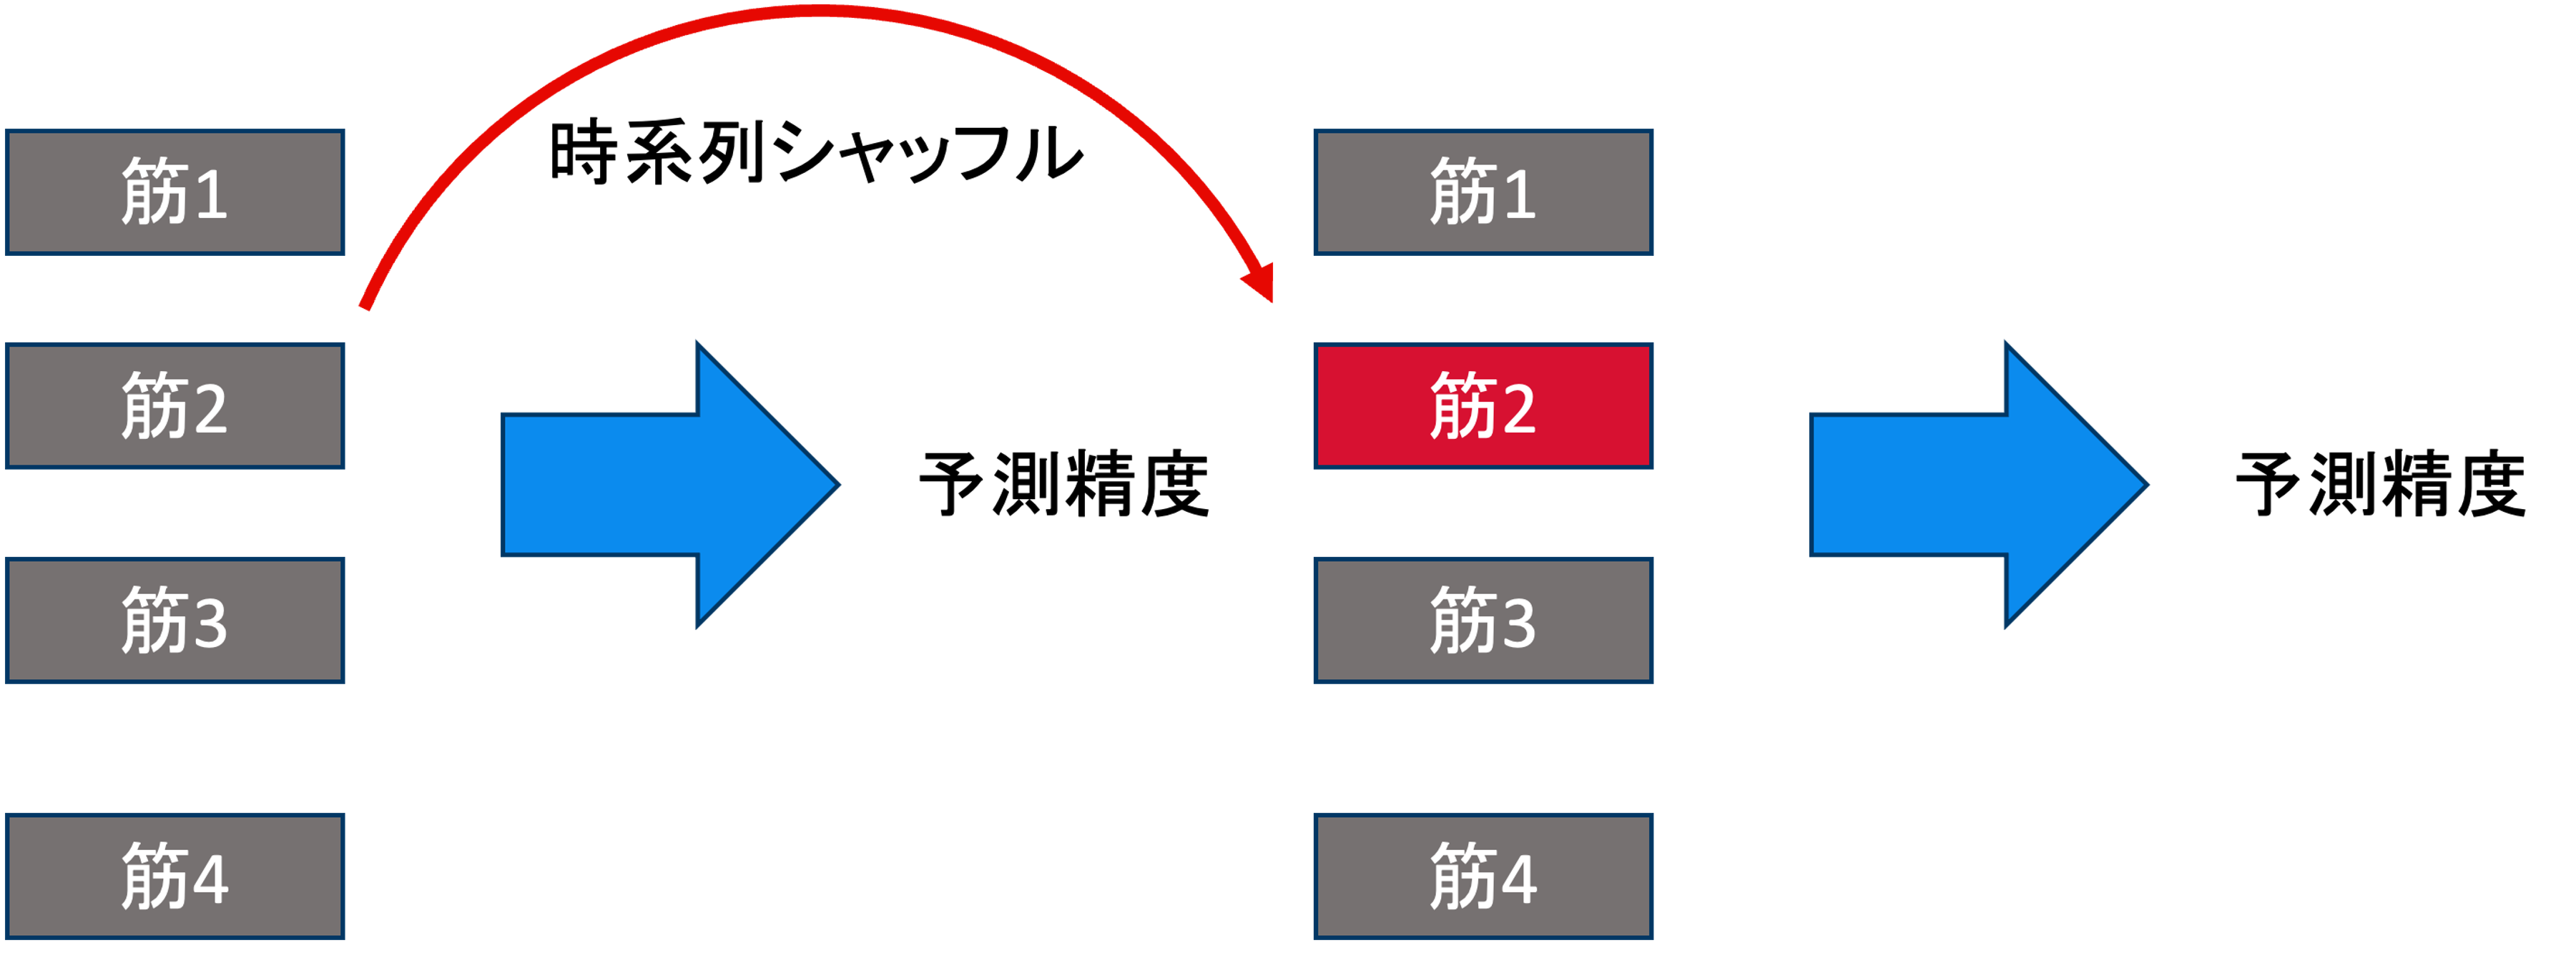
\includegraphics[keepaspectratio, width=1.0\linewidth]{chap1/PFI.png}
  \caption{PFIの手法説明}
  \label{fig:PFI}
\end{figure}

\section{本研究の目的}
\label{sec:intro_my_purpose}
1.1節で述べたように，パラアスリートの身体機能には極めて大きな多様性が存在するため，従来のスポーツ科学における一般化（集団の平均モデル）のアプローチを適用することには限界がある．
選手のパフォーマンスを最大化するためには，個別最適化のアプローチへと転換する必要がある．

一方，1.2節で概観したように，車椅子卓球に関する先行研究の多くは，身体の動き（キネマティクス）や単発の動作解析に留まっている．
動作の駆動源である筋活動や，実際の試合で重要となる連続的なラリーを考慮した解析は十分になされておらず，指導現場で活用できる客観的な指標は確立されていない．
そこで，本研究の目的を以下の通りに設定する．

% textlint-disable ja-technical-writing/ja-no-mixed-period

\bigskip
\begin{itembox}[c]{目的}
  \centering
車椅子卓球のラリー中の打球精度に寄与する身体動作および筋活動の解析
\end{itembox}

% textlint-enable ja-technical-writing/ja-no-mixed-period

\clearpage

\section{本論文の構成}
\label{sec:configuration}

本論文は，全\ref{cp:conclusion}章から構成されている．
%本論文の構成を\reffig{fig:configuration}に示す．

\refcp{cp:introduction}では，本研究の背景と先行研究，目的について述べた．

\refcp{cp:proposed_method}では，本研究における車椅子卓球選手の競技中の動作の測定と解析のアプローチについて述べる．

\refcp{cp:verification_experiment}では，車椅子卓球選手のパフォーマンスを左右する要因について解析を行い，その結果，考察について述べる．

\refcp{cp:conclusion}では，本論文の結論と今後の展望を述べる．

% \vspace{3\zh}
% \begin{figure}[h]
%   \centering
%   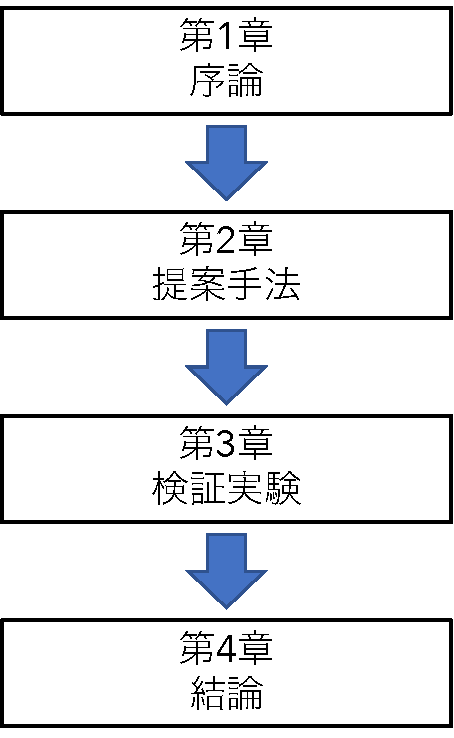
\includegraphics[keepaspectratio, width=0.35\linewidth]{chap1/configuration.pdf}
%   \caption{本論文の構成}
%   \label{fig:configuration}
% \end{figure}

\clearpage

\end{document}
